\chapter{Metodologia}
% ---
% ---
Neste segmento, serão delineadas informações relacionadas à elaboração da aplicação proposta neste projeto. Discutiremos a estruturação do desenvolvimento e a análise de requisitos, abrangendo tanto os funcionais quanto os não funcionais.

Na delineação da Estruturação do desenvolvimento, é vital compreender a sinergia entre os componentes, visando otimizar a eficiência e a coesão do sistema em questão. Os requisitos funcionais, sendo pilares fundamentais, demandam uma abordagem analítica aprimorada para assegurar sua implementação fluída.

Quanto aos requisitos não funcionais, devemos explorar suas nuances de maneira minudente, reconhecendo a importância intrínseca de cada faceta no contexto global do projeto. Esta abordagem detalhada proporciona uma compreensão mais profunda, permitindo a delimitação precisa de parâmetros que transcendem as fronteiras meramente operacionais.

\section{Estruturação do desenvolvimento}\label{sec:estruturacao-desenvolvimento}
A forma como foi organizado o desenvolvimento do presente trabalho consiste inicialmente em pesquisas exploratórias realizadas através de entrevistas conduzidas com um membro da Brigada Militar, SD. Tiago Costa. Durante essas entrevistas, foram formuladas perguntas pertinentes ao procedimento de geração do AEL.

A coleta de informações foi complementada por meio de análise documental, sendo como principal embasamento a Portaria 136 de 8 de novembro de 2019 do Exército Brasileiro, mais especificamente o anexo D do \citeonline{ExércitoBrasileiro} constante nos Anexos (\ref{sec:anexoA1}, \ref{sec:anexoA2}, \ref{sec:anexoA3}, \ref{sec:anexoA4}). Esta documentação conceitua todas as fases envolvidas no processo de geração do AEL da Brigada Militar do Rio Grande do Sul.

A partir da análise de escopo realizada, planejou-se o uso do modelo de desenvolvimento iterativo neste projeto pois de acordo com \citeonline{engenhariasw}, se um processo interno de desenvolvimento iterativo é usado, o documento de requisitos pode ser muito menos detalhado e quaisquer ambiguidades podem ser resolvidas durante o desenvolvimento do sistema.

Logo a complexidade do procedimento de geração do AEL demanda uma abordagem flexível, permitindo ajustes contínuos à medida que novos pontos de vista são revelados durante entrevistas com SD. Tiago Costa. Essa metodologia proporciona validação incremental das fases, adaptabilidade a mudanças nos requisitos e envolvimento constante, garantindo um desenvolvimento mais preciso.


\section{Análise de Requisitos}
Os requisitos inerentes a aplicação web, foram levantados com base nas informações coletadas durantes as reuniões com os envolvidos conforme citado na \autoref{sec:estruturacao-desenvolvimento} sendo avaliado como as funcionalidades essenciais aquelas que impactam diretamente o pleno funcionamento da aplicação, quais devem ser implementadas durante o desenvolvimento do sistema. Ademais, foi realizada uma avaliação para determinar as funcionalidades desejáveis.

Sendo divida esta em subseções contendo os requisitos funcionais e não funcionais.

\subsection{Requisitos Funcionais}
Nesta subseção, será abordado os requisitos funcionais, aqueles que abrangem e descrevem todas as funcionalidades previstas para o sistema. 

\begin{table}[H]\label{tab:rf01}
    \caption{Requisito Funcional 1}
    \centering
    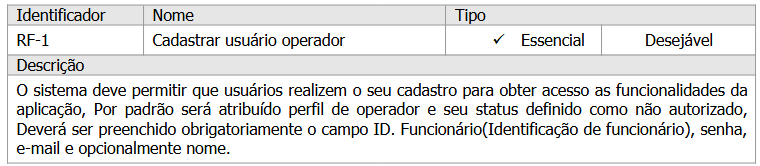
\includegraphics[scale=0.82]{imagens/rf01.png}
    \legend{Fonte: Autor}
\end{table}
\begin{table}[H]\label{tab:rf02}
    \caption{Requisito Funcional 2}
    \centering
    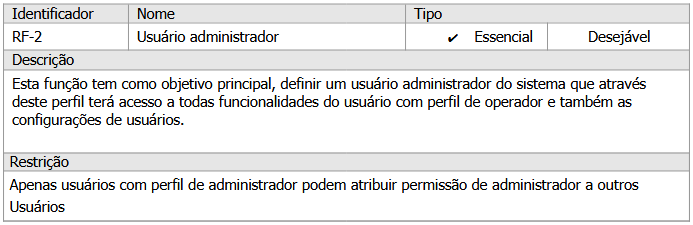
\includegraphics[scale=0.82]{imagens/rf02.png}
    \legend{Fonte: Autor}
\end{table}
\begin{table}[H]\label{tab:rf03}
    \caption{Requisito Funcional 3}
    \centering
    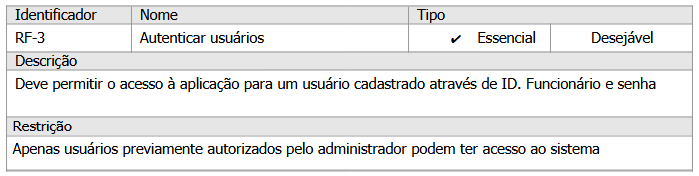
\includegraphics[scale=0.9]{imagens/rf03.png}
    \legend{Fonte: Autor}
\end{table}
\begin{table}[H]\label{tab:rf04}
    \caption{Requisito Funcional 4}
    \centering
    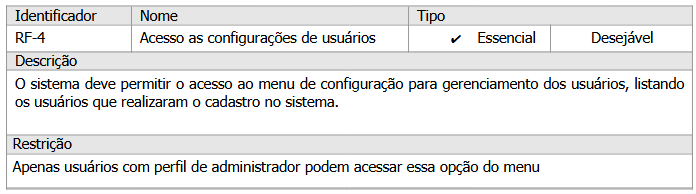
\includegraphics[scale=0.9]{imagens/rf04.png}
    \legend{Fonte: Autor}
\end{table}
\begin{table}[H]\label{tab:rf05}
    \caption{Requisito Funcional 5}
    \centering
    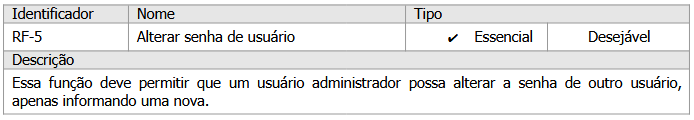
\includegraphics[scale=0.9]{imagens/rf05.png}
    \legend{Fonte: Autor}
\end{table}
\begin{table}[H]
    \caption{Requisito Funcional 6}\label{tab:rf06}
    \centering
    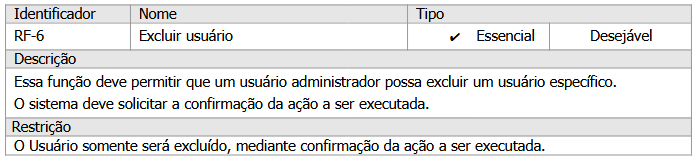
\includegraphics[scale=0.9]{imagens/rf06.png}
    \legend{Fonte: Autor}
\end{table}
\begin{table}[H]
    \caption{Requisito Funcional 7}\label{tab:rf07}
    \centering
    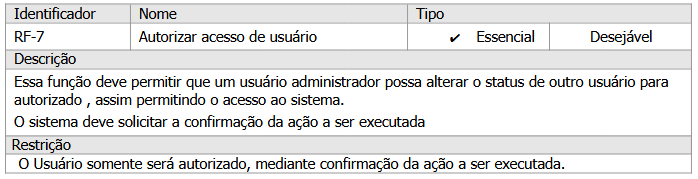
\includegraphics[scale=0.9]{imagens/rf07.png}
    \legend{Fonte: Autor}
\end{table}
\begin{table}[H]
    \caption{Requisito Funcional 8}\label{tab:rf08}
    \centering
    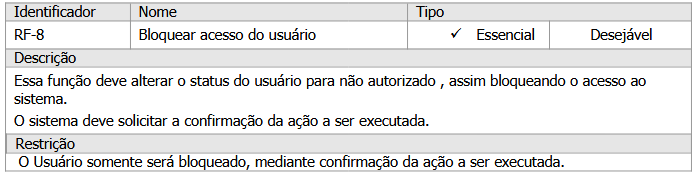
\includegraphics[scale=0.9]{imagens/rf08.png}
    \legend{Fonte: Autor}
\end{table}
\begin{table}[H]
    \caption{Requisito Funcional 9}\label{tab:rf09}
    \centering
    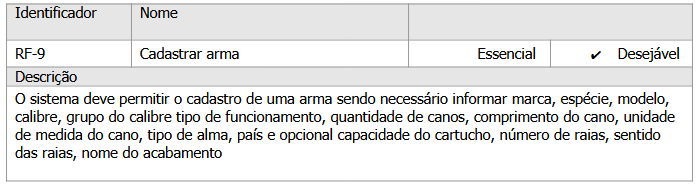
\includegraphics[scale=0.9]{imagens/rf09.png}
    \legend{Fonte: Autor}
\end{table}
\begin{table}[H]
    \caption{Requisito Funcional 10}\label{tab:rf10}
    \centering
    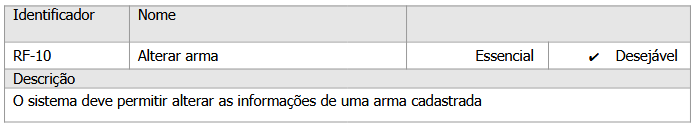
\includegraphics[scale=0.9]{imagens/rf10.png}
    \legend{Fonte: Autor}
\end{table}
\begin{table}[H]
    \caption{Requisito Funcional 11}\label{tab:rf11}
    \centering
    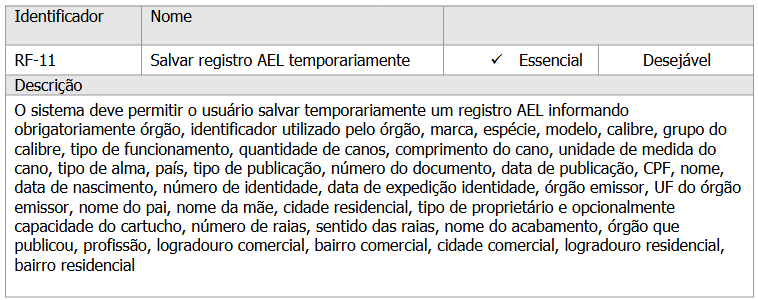
\includegraphics[scale=0.82]{imagens/rf11.png}
    \legend{Fonte: Autor}
\end{table}
\begin{table}[H]
    \caption{Requisito Funcional 12}\label{tab:rf12}
    \centering
    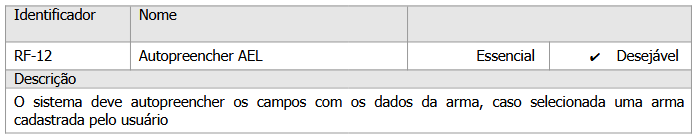
\includegraphics[scale=0.9]{imagens/rf12.png}
    \legend{Fonte: Autor}
\end{table}
\begin{table}[H]
    \caption{Requisito Funcional 13}\label{tab:rf13}
    \centering
    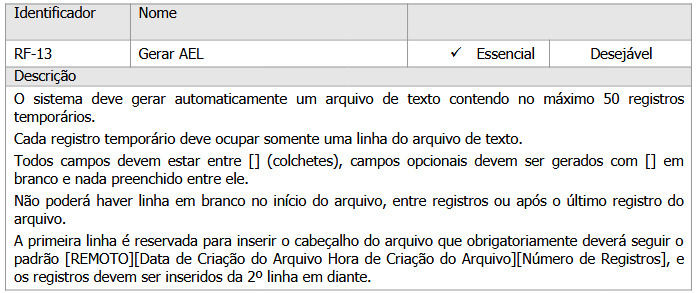
\includegraphics[scale=0.9]{imagens/rf13.png}
    \legend{Fonte: Autor}
\end{table}
\begin{table}[H]
    \caption{Requisito Funcional 14}\label{tab:rf14}
    \centering
    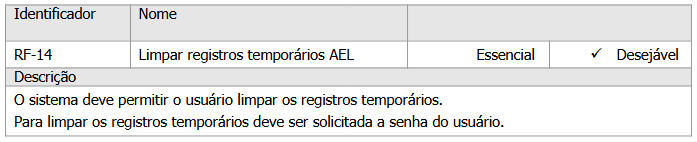
\includegraphics[scale=0.9]{imagens/rf14.png}
    \legend{Fonte: Autor}
\end{table}



\subsection{Requisitos Não Funcionais}
Na presente subseção, serão apresentados os requisitos não funcionais da aplicação, os quais descrevem as características globais do sistema, indo além das funcionalidades específicas.
E assegurando uma compreensão completa e abrangente dos métodos empregados pela aplicação para alcançar o resultado almejado.

\begin{table}[H]
    \caption{Requisito Não Funcional 1}\label{tab:rnf1}
    \centering
    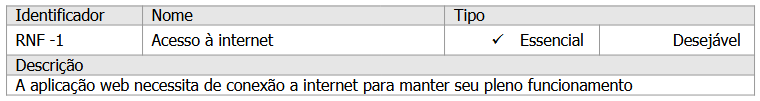
\includegraphics[scale=0.82]{imagens/rnf1.png}
    \legend{Fonte: Autor}
\end{table}
\begin{table}[H]
    \caption{Requisito Não Funcional 2}\label{tab:rnf2}
    \centering
    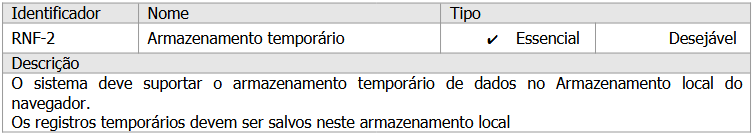
\includegraphics[scale=0.82]{imagens/rnf2.png}
    \legend{Fonte: Autor}
\end{table}
\begin{table}[H]
    \caption{Requisito Não Funcional 3}\label{tab:rnf3}
    \centering
    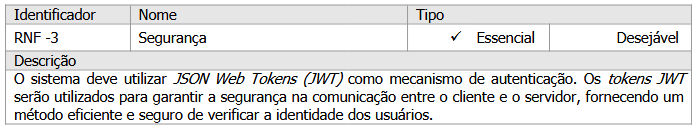
\includegraphics[scale=0.82]{imagens/rnf3.png}
    \legend{Fonte: Autor}
\end{table}
\begin{table}[H]
    \caption{Requisito Não Funcional 4}\label{tab:rnf4}
    \centering
    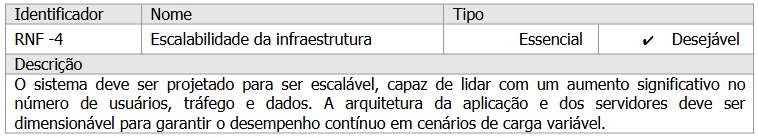
\includegraphics[scale=0.82]{imagens/rnf4.png}
    \legend{Fonte: Autor}
\end{table}
\begin{table}[H]
    \caption{Requisito Não Funcional 5}\label{tab:rnf5}
    \centering
    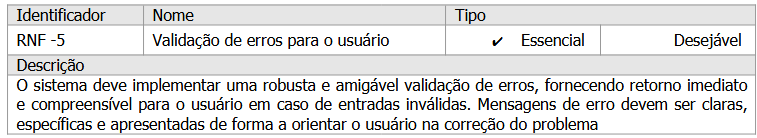
\includegraphics[scale=0.82]{imagens/rnf5.png}
    \legend{Fonte: Autor}
\end{table}
\begin{table}[H]
    \caption{Requisito Não Funcional 6}\label{tab:rnf6}
    \centering
    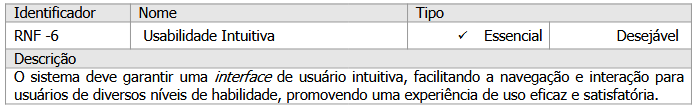
\includegraphics[scale=0.82]{imagens/rnf6.png}
    \legend{Fonte: Autor}
\end{table}
% % ---
% \section{Tabelas}
% % ---

% \index{tabelas}A \autoref{tab-nivinv} é um exemplo de tabela construída em
% \LaTeX.

% \begin{table}[htb]
% \ABNTEXfontereduzida
% \caption[Níveis de investigação]{Níveis de investigação.}
% \label{tab-nivinv}
% \begin{tabular}{p{2.6cm}|p{6.0cm}|p{2.25cm}|p{3.40cm}}
%   %\hline
%    \textbf{Nível de Investigação} & \textbf{Insumos}  & \textbf{Sistemas de Investigação}  & \textbf{Produtos}  \\
%     \hline
%     Meta-nível & Filosofia\index{filosofia} da Ciência  & Epistemologia &
%     Paradigma  \\
%     \hline
%     Nível do objeto & Paradigmas do metanível e evidências do nível inferior &
%     Ciência  & Teorias e modelos \\
%     \hline
%     Nível inferior & Modelos e métodos do nível do objeto e problemas do nível inferior & Prática & Solução de problemas  \\
%    % \hline
% \end{tabular}
% \legend{Fonte: \citeonline{van86}}
% \end{table}

% Já a \autoref{tabela-ibge} apresenta uma tabela criada conforme o padrão do
% \citeonline{ibge1993} requerido pelas normas da ABNT para documentos técnicos e
% acadêmicos.

% \begin{table}[htb]
% \IBGEtab{%
%   \caption{Um Exemplo de tabela alinhada que pode ser longa
%   ou curta, conforme padrão IBGE.}%
%   \label{tabela-ibge}
% }{%
%   \begin{tabular}{ccc}
%   \toprule
%    Nome & Nascimento & Documento \\
%   \midrule \midrule
%    Maria da Silva & 11/11/1111 & 111.111.111-11 \\
%   \midrule 
%    João Souza & 11/11/2111 & 211.111.111-11 \\
%   \midrule 
%    Laura Vicuña & 05/04/1891 & 3111.111.111-11 \\
%   \bottomrule
% \end{tabular}%
% }{%
%   \fonte{Produzido pelos autores.}%
%   \nota{Esta é uma nota, que diz que os dados são baseados na
%   regressão linear.}%
%   \nota[Anotações]{Uma anotação adicional, que pode ser seguida de várias
%   outras.}%
%   }
% \end{table}
% ---


